%!TEX TS-program = xelatex
\documentclass[12pt, a4paper, oneside]{article}

\usepackage{amsmath,amsfonts,amssymb,amsthm,mathtools}  % пакеты для математики

\usepackage[english, russian]{babel} % выбор языка для документа
\usepackage[utf8]{inputenc} % задание utf8 кодировки исходного tex файла
\usepackage[X2,T2A]{fontenc}        % кодировка

\usepackage{fontspec}         % пакет для подгрузки шрифтов
\setmainfont{Linux Libertine O}   % задаёт основной шрифт документа

\usepackage{unicode-math}     % пакет для установки математического шрифта
\setmathfont[math-style=upright]{Neo Euler} % шрифт для математики

% Конкретный символ из конкретного шрифта
% \setmathfont[range=\int]{Neo Euler}

%%%%%%%%%% Работа с картинками %%%%%%%%%
\usepackage{graphicx}                  % Для вставки рисунков
\usepackage{graphics}
\graphicspath{{images/}{pictures/}}    % можно указать папки с картинками
\usepackage{wrapfig}                   % Обтекание рисунков и таблиц текстом

%%%%%%%%%%%%%%%%%%%%%%%% Графики и рисование %%%%%%%%%%%%%%%%%%%%%%%%%%%%%%%%%
\usepackage{tikz, pgfplots}  % язык для рисования графики из latex'a

%%%%%%%%%% Гиперссылки %%%%%%%%%%
\usepackage{xcolor}              % разные цвета

\usepackage{hyperref}
\hypersetup{
	unicode=true,           % позволяет использовать юникодные символы
	colorlinks=true,       	% true - цветные ссылки, false - ссылки в рамках
	urlcolor=blue,          % цвет ссылки на url
	linkcolor=red,          % внутренние ссылки
	citecolor=green,        % на библиографию
	pdfnewwindow=true,      % при щелчке в pdf на ссылку откроется новый pdf
	breaklinks              % если ссылка не умещается в одну строку, разбивать ли ее на две части?
}


\usepackage{todonotes} % для вставки в документ заметок о том, что осталось сделать
% \todo{Здесь надо коэффициенты исправить}
% \missingfigure{Здесь будет Последний день Помпеи}
% \listoftodos --- печатает все поставленные \todo'шки

\usepackage[paper=a4paper, top=20mm, bottom=15mm,left=20mm,right=15mm]{geometry}
\usepackage{indentfirst}       % установка отступа в первом абзаце главы

\usepackage{setspace}
\setstretch{1.15}  % Межстрочный интервал
\setlength{\parskip}{4mm}   % Расстояние между абзацами
% Разные длины в латехе https://en.wikibooks.org/wiki/LaTeX/Lengths


\usepackage{xcolor} % Enabling mixing colors and color's call by 'svgnames'

\definecolor{MyColor1}{rgb}{0.2,0.4,0.6} %mix personal color
\newcommand{\textb}{\color{Black} \usefont{OT1}{lmss}{m}{n}}
\newcommand{\blue}{\color{MyColor1} \usefont{OT1}{lmss}{m}{n}}
\newcommand{\blueb}{\color{MyColor1} \usefont{OT1}{lmss}{b}{n}}
\newcommand{\red}{\color{LightCoral} \usefont{OT1}{lmss}{m}{n}}
\newcommand{\green}{\color{Turquoise} \usefont{OT1}{lmss}{m}{n}}

\usepackage{titlesec}
\usepackage{sectsty}
%%%%%%%%%%%%%%%%%%%%%%%%
%set section/subsections HEADINGS font and color
\sectionfont{\color{MyColor1}}  % sets colour of sections
\subsectionfont{\color{MyColor1}}  % sets colour of sections

%set section enumerator to arabic number (see footnotes markings alternatives)
\renewcommand\thesection{\arabic{section}.} %define sections numbering
\renewcommand\thesubsection{\thesection\arabic{subsection}} %subsec.num.

%define new section style
\newcommand{\mysection}{
	\titleformat{\section} [runin] {\usefont{OT1}{lmss}{b}{n}\color{MyColor1}} 
	{\thesection} {3pt} {} } 


%	CAPTIONS
\usepackage{caption}
\usepackage{subcaption}
%%%%%%%%%%%%%%%%%%%%%%%%
\captionsetup[figure]{labelfont={color=Turquoise}}

\pagestyle{empty}

\begin{document}
	
\section*{Семинар 4-5: Продажи и линейная регрессия }

\subsection*{Задача 1}

Предположим, Олег хочет купить автомобиль и считает сколько денег ему нужно для этого накопить\footnote{сделано по мотивам \url{https://vas3k.ru/blog/machine_learning/}}. Он пересмотрел десяток объявлений в интернете и увидел, что новые автомобили стоят около $20 000$, годовалые — примерно $19 000$, двухлетние — $18 000$ и так далее.

В уме Олег-аналитик выводит формулу: адекватная цена автомобиля начинается от $20 000$ и падает на $1000$ каждый год, пока не упрётся в $10 000$. Олег сделал то, что в машинном обучении называют регрессией — предсказал цену по известным данным. Давайте попробуем повторить подвиг Олега.

\begin{enumerate}
	\item Как выглядит формула в случае Олега?
	\item За сколько продать старый афон? Как выглядит формула?
	\item Сколько шашлыка брать на дачу? Как выглядит формула?
	\item Сколько брать шашлыка, если есть толстый друг? Как можно назвать толстого друга в терминах машинного обучения? Испортит ли толстый друг формулу?
	\item Сколько одежды брать с собой в путешествие? (тут они начнут рассуждать что это зависит не только от срока путешествия, но и от пола и бац у нас уже много факторов)
\end{enumerate}

Было бы удобно иметь формулу под каждую проблему на свете. Но взять те же цены на автомобили: кроме пробега есть десятки комплектаций, разное техническое состояние, сезонность спроса и еще столько неочевидных факторов, которые Олег, даже при всём желании, не учел бы в голове. Люди тупы и ленивы — надо заставить вкалывать роботов.

\subsection*{Задача 2}

Вот несколько ситуаций, как на ваш взгляд должны пройти линии регрессии? Да, это тоже машинное обучение. Но обычно кривые рисуем не мы, а комплюхтер.

\begin{minipage}[t]{0.45\textwidth}
	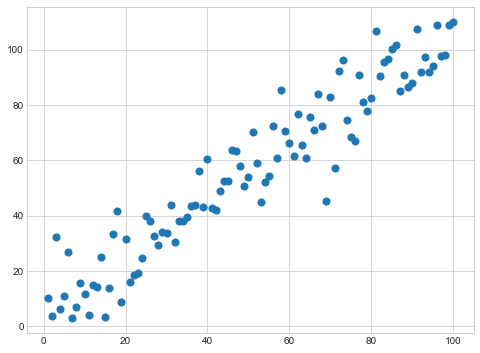
\includegraphics[scale=0.4]{regr_pic_1.png}
\end{minipage}
\hfill
\begin{minipage}[t]{0.45\textwidth}
	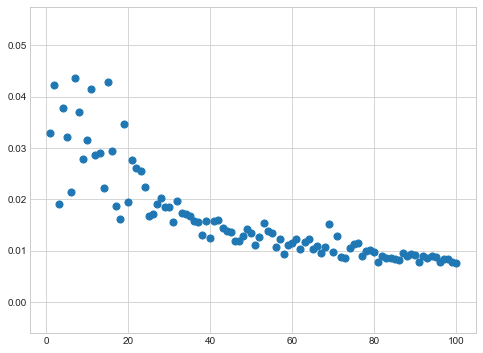
\includegraphics[scale=0.4]{regr_pic_2.png}
\end{minipage}

\begin{minipage}[t]{0.45\textwidth}
	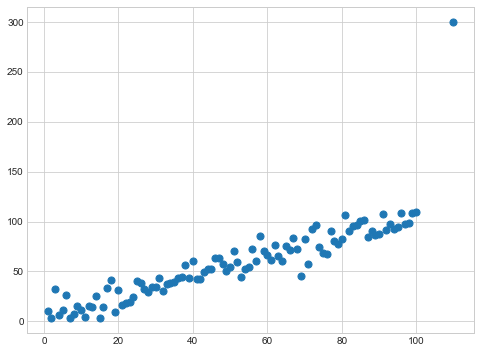
\includegraphics[scale=0.4]{regr_pic_3.png}
\end{minipage}
\hfill
\begin{minipage}[t]{0.45\textwidth}
	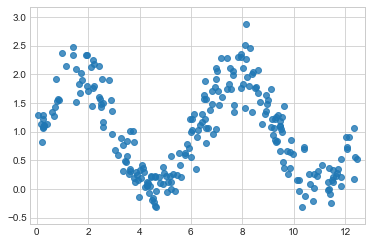
\includegraphics[scale=0.55]{regr_pic_4.png}
\end{minipage}

\begin{enumerate}	
	\item Нарисуйте на каждой из картинок линию регрессии.
	\item Как выглядят уравнения регрессии в этих ситуациях? Какие параметры в них нам нужно обучить?
	\item В чём проблема на картинке слева снизу? Проинтерпретируйте её на примере шашлыков.
	\item Поговорить про полином и переобучение.
	\item Как будет выглядеть рисунок, если $y$ — сколько вещей надо брать с собой в путешествие, $x_1$ — время поездки, $x_2$ — пол путешественника.
	\item Ещё одна, на этот раз трёхмерная картинка! Слабо дополнить её также, как мы делали это выше? Как будет выглядеть уравнение регрессии?
\end{enumerate}

\begin{center}
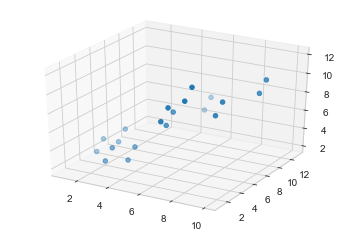
\includegraphics[scale=0.8]{regr_pic_5.png}
\end{center}


\subsection*{Задача 3}

Вася измерил вес трёх упаковок с конфетками,  $y_1=6$, $y_2=6$, $y_3=10$.  Вася хочет спрогнозировать вес следующего пакетика. Модель для веса пакетиков у Васи очень простая, $y_i = \mu + u_i$, поэтому прогнозирует Вася по формуле $\hat y_i = \hat \mu$.

Для оценки параметра $\mu$ Вася использует следующую целевую функцию:
\[
\sum (y_i - \hat \mu)^2 + \lambda \cdot \hat \mu^2
\]

\begin{enumerate}
	\item Найдите оптимальное $\hat\mu$ при $\lambda =0$.
	\item Найдите оптимальное $\hat\mu$ при произвольном $\lambda$.
	\item Подберите оптимальное $\lambda$ с помощью кросс-валидации «выкинь одного».
	\item Найдите оптимальное $\hat\mu$ при $\lambda_{CV}$.
\end{enumerate}


%	$\hat\mu_{\lambda=0}=22/3$
%	При минимизации $RSS^{CV}$ разумно сделать замену $t=4/(2+\lambda)$, тогда $RSS^{CV}=2(6-4t)2+(10-3t)^2$.
%	$\lambda_{CV} = 4/39$, $\hat\mu = \frac{22}{3+4/39}$


\subsection*{Задача 4}

Миша работает в маленькой кофейне. Харио Малабар Монсун является фирменным напитком этой кофейни. Мише интересно узнать как именно ведёт себя спрос на напиток $y_i$ в зависимости от температуры за окном $t_i$. Четыре дня Миша записывал свои наблюдения: 

\begin{center}
	\begin{tabular}{c|c}
		\hline
		$t_i$ & $y_i$ \\
		\hline
		21 &  1 \\
		19 & 2 \\
		12 & 8 \\
	     8 & 8 \\
	\end{tabular}
\end{center}

Сегодня он решил обучить регрессионное дерево. В качестве функции потерь он использует 

\[ \sum (y_i - \hat y_i)^2. \]

\begin{enumerate}
	\item Обучите регрессионное дерево.
	\item Какой прогноз на сегодня сделает дерево Миши, если за окном $13$ градусов? 
\end{enumerate}


\subsection*{Задача 5}

Предположим, что в наших руках оказались исторические данные по продажам $45$ магазинов Walmart, расположенных в разных регионах. Каждый магазан содержит несколько отделов.  Нам хотелось бы научиться прогнозировать продажи по каждому отделу. 

\begin{enumerate}
	\item  Зачем нам может понадобиться прогнозировать продажи? Какая от этого выгода для магазина? 
	\item Какую задачу машинного обучения нам предстоит решать? Какие переменные мы могли бы использовать в качестве объясняющих? 
	\item Какую метрику мы могли бы использовать для оценки бизнес-эффекта от нашей модели? Отталкиваясь от каких характеристик можно было бы сконструировать её? 
	\item  Что такое MAE, MSE,  RMSE и MAPE?  Предположим, что у нас есть три магазина. Они продали товаров на $5$, $10$ и $100$  рублей.  Наша модель предсказывала, что они продадут товаров на  $4$, $20$ и $110$. Посчитайте для нашей модели все четыре метрики качества, приведённые выше. 
\end{enumerate}


\section*{Ещё задачи}

\subsection*{Задача 6}

Маркетологи Вова и Вася строили регрессию $y = \beta_0 + \beta_1 x$. Каждый оценивал её по своим данным. У Васи получилось, что $\hat \beta_1 = 2$, у Вовы получилось, что $\hat \beta_1 = 8$.

Пришла Алиса, отобрала у Вовы и Васи данные, соединила их вместе и построила регрессию сразу на всём. У неё получилось, что $\hat \beta_1 = -10$. Может ли такое быть?

\subsection*{Задача 7}

Выращиваем регрессионное дерево в домашних условиях! Вот вам выборка для этого: 

\begin{center}
	\begin{tabular}{c|c}
		\hline
		$x_i$ & $y_i$ \\
		\hline
		0 & 5 \\
		1 &  6\\
		2 & 4 \\
		3 & 100 \\
	\end{tabular}
\end{center}

Критерий деления вершины --- минимизация квадратичной функции потерь. Критерий остановки --- три листа.  Зачем нужен критерий остановки? Как дерево ведёт себя с выбросами? 

\subsection*{Задача 8}

Каждый день Маша ест конфеты и решает задачи по машинному обучению. Пусть $x_i$ — количество решённых задач, а $y_i$ — количество съеденных конфет.

\begin{center}
\begin{tabular}{c|c}
	\hline
	$x_i$ & $y_i$ \\
	\hline
	1 & 1 \\
	2 & 2 \\
	2 & 8 \\
\end{tabular}
\end{center}

Рассмотрим модель $y_i = \beta x_i + u_i$. Маша использует функцию потерь 
\[
\sum (y_i - \hat \beta x_i )^2
\]

\begin{enumerate}
	\item Найдите МНК-оценку $\hat b$ для имеющихся трёх наблюдений.
	\item Нарисуйте исходные точки и полученную прямую
	регрессии.
	\item Выведите формулу для $\hat b$ в общем виде для $n$ наблюдений.
	\item На семинаре по машинному обучению неожиданно выяснилось, что Миша тоже каждый день решает задачи по машинному обучению. Правда он более сдержан в плане конфет. Миша решил взять Машины наблюдения и с помощью функционала 
	\[
	\sum |y_i - \hat \beta x_i |
	\]  
	
	оценить $\beta$. Помогите Мише найти оценку. 
	\item К поеданию конфет решает присоединиться Вадик. У него тоже есть своя функция потерь
	\[
	\sum (y_i - \hat \beta x_i)^2 + 3\beta^2
	\]  	
	Оцените $\beta$ для его случая. Нарисуйте все три прямые на одной картинке и порассуждайте почему они получились именно такими, какими получились. 
\end{enumerate}

\end{document}
